Take $x_{it} $ fo which $\overline{x_i} = x_{it}, \forall i, t.$

\begin{theorem}[Hausman-Test]\label{Hausman-test}
    \
    
    $\mathcal{H}_0$: $\hat{\beta}_{RE, pop} = \hat{\beta}_{FE-W, pop}$ $\Leftrightarrow$ We should use $\hat{\beta}_{RE}$.

    We define:
    \begin{align*}
        T_{Hausman} &= n \Bigl(\hat{\beta}_{FE} - \hat{\beta}_{RE} \Bigr)^{\prime} \Bigl( A\mathbb{V}[\hat{\beta}_{FE}] - A\mathbb{V}[\hat{\beta}_{RE}] \Bigr)^{-1} \Bigl(\hat{\beta}_{FE} - \hat{\beta}_{RE}\Bigr) \rightarrow \chi_k^2
    \end{align*}
\end{theorem}

\begin{note}
    \

    To sum up, the FE estimators work under arbitrary correlation between the unobserved
heterogeneity $\alpha_i$ and covariates $X_i$ , but they cannot deal with time-constant regressors and
their consistency is paid for by an efficiency loss relative to RE estimators.

    Most importantly, their consistency requires strict exogeneity, 
    a much stronger assumption than contemporaneous exogeneity of covariates and error terms.
\end{note}

\subsection{FE-IV Estimation}

\begin{enumerate}
    \item Contemperaneous exogeneity: $\mathbb{E}[x_{it} u_{it}] = 0, \forall t.$
    \item Strict exogeneity: $\mathbb{E}[x_{it} u_{is}] = 0, \forall t, s.$
    \item Sequential exogeneity: $\mathbb{E}[x_{it} u_{is}] = 0, \forall t, s \geq t.$
    \begin{definition}[Predetermined variables(Or Sequantial Exogeneity)]
        \

        Predetermined variables are variables that were determined prior to the current period. 
        In econometric models this implies that the current period error term is 
        uncorrelated with current and lagged values of the predetermined variable 
        but may be correlated with future values. 
        This is a weaker restriction than strict exogeneity, 
        which requires the variable to be uncorrelated with past, present, and future shocks.
    \end{definition}
\end{enumerate}

Still assume that we have a standard model:
\begin{align*}
    y_{it} &= \alpha_i + x_{it}^{\prime} \beta + u_{it} \\
    &= \alpha_i + \beta_1 y_{i, t-1} + \tilde{x}_{it}^{\prime} \beta_{-1} + u_{it}  \\
    \Rightarrow \Delta y_{it} &= \Delta \alpha_i + \Delta x_{it}^{\prime} \beta + \Delta u_{it}
\end{align*}
\begin{definition}[Anderson and Hsiao(1981)]
    \

    FE-IV: Use $y_{i,t-2}$ as the IV for $\Delta y_{i,t-1}$.

    Under sequential exogeneity, instrument-exogeneity is satisied:
    \[\mathbb{E}[y_{is} \Delta u_{it}] = 0, \forall s\leq t-2.\]
\end{definition}

\begin{figure}[htbp!]
    \centering
    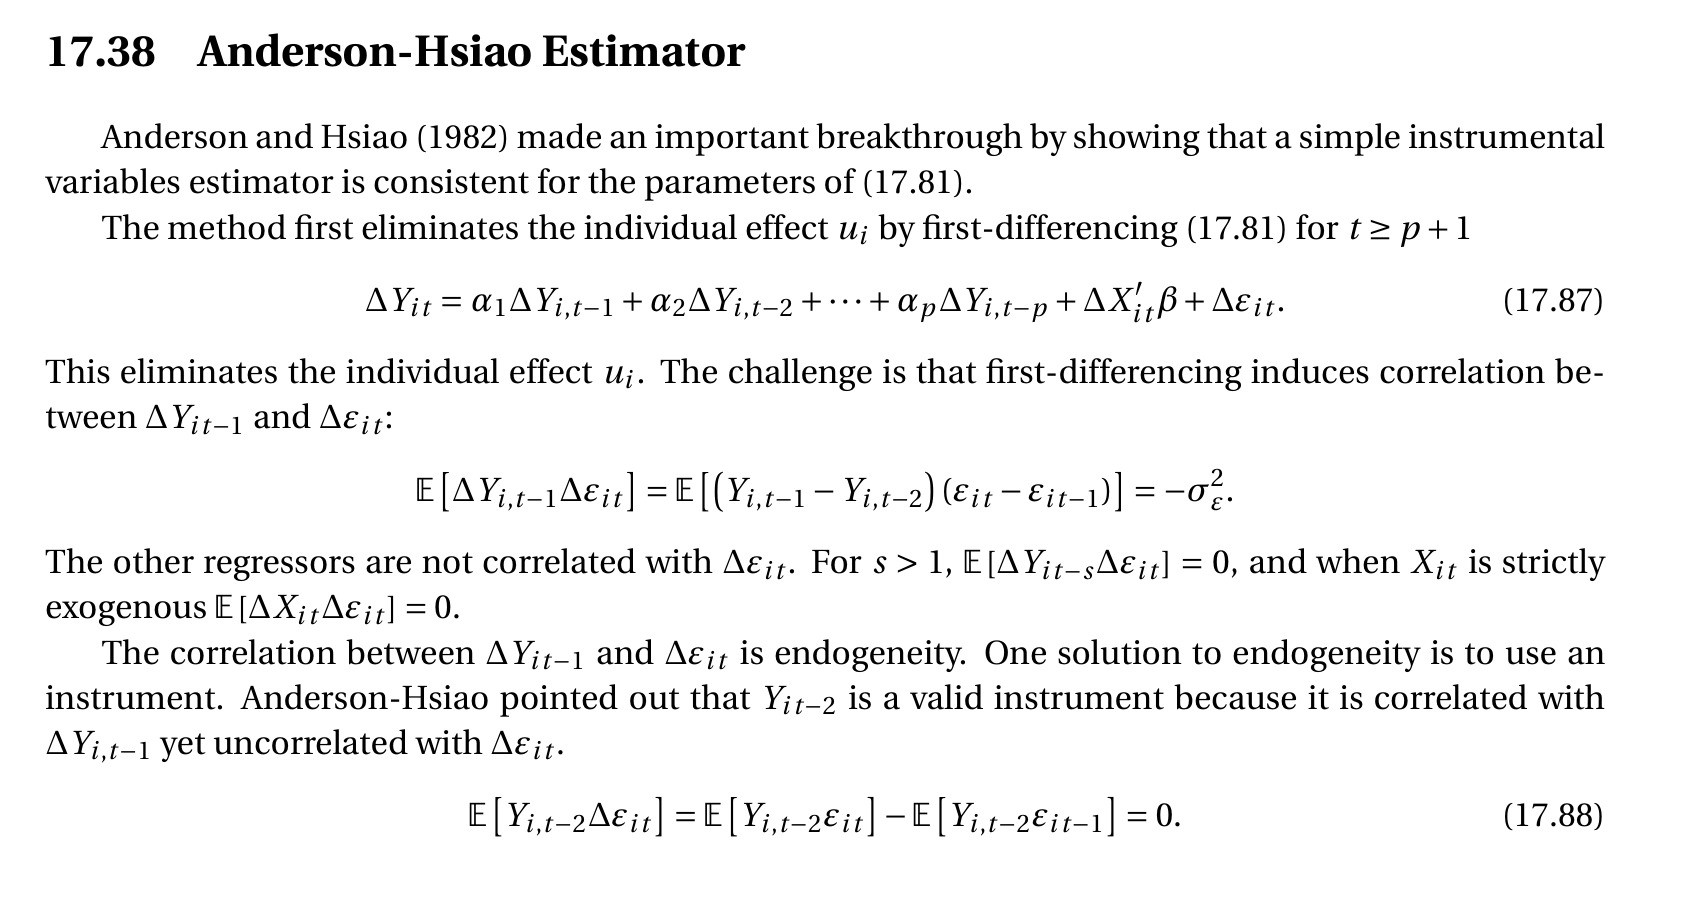
\includegraphics[width=\linewidth]{figures/Anderson-Hsiao-1981.png}
\end{figure}
\begin{figure}
    \centering
    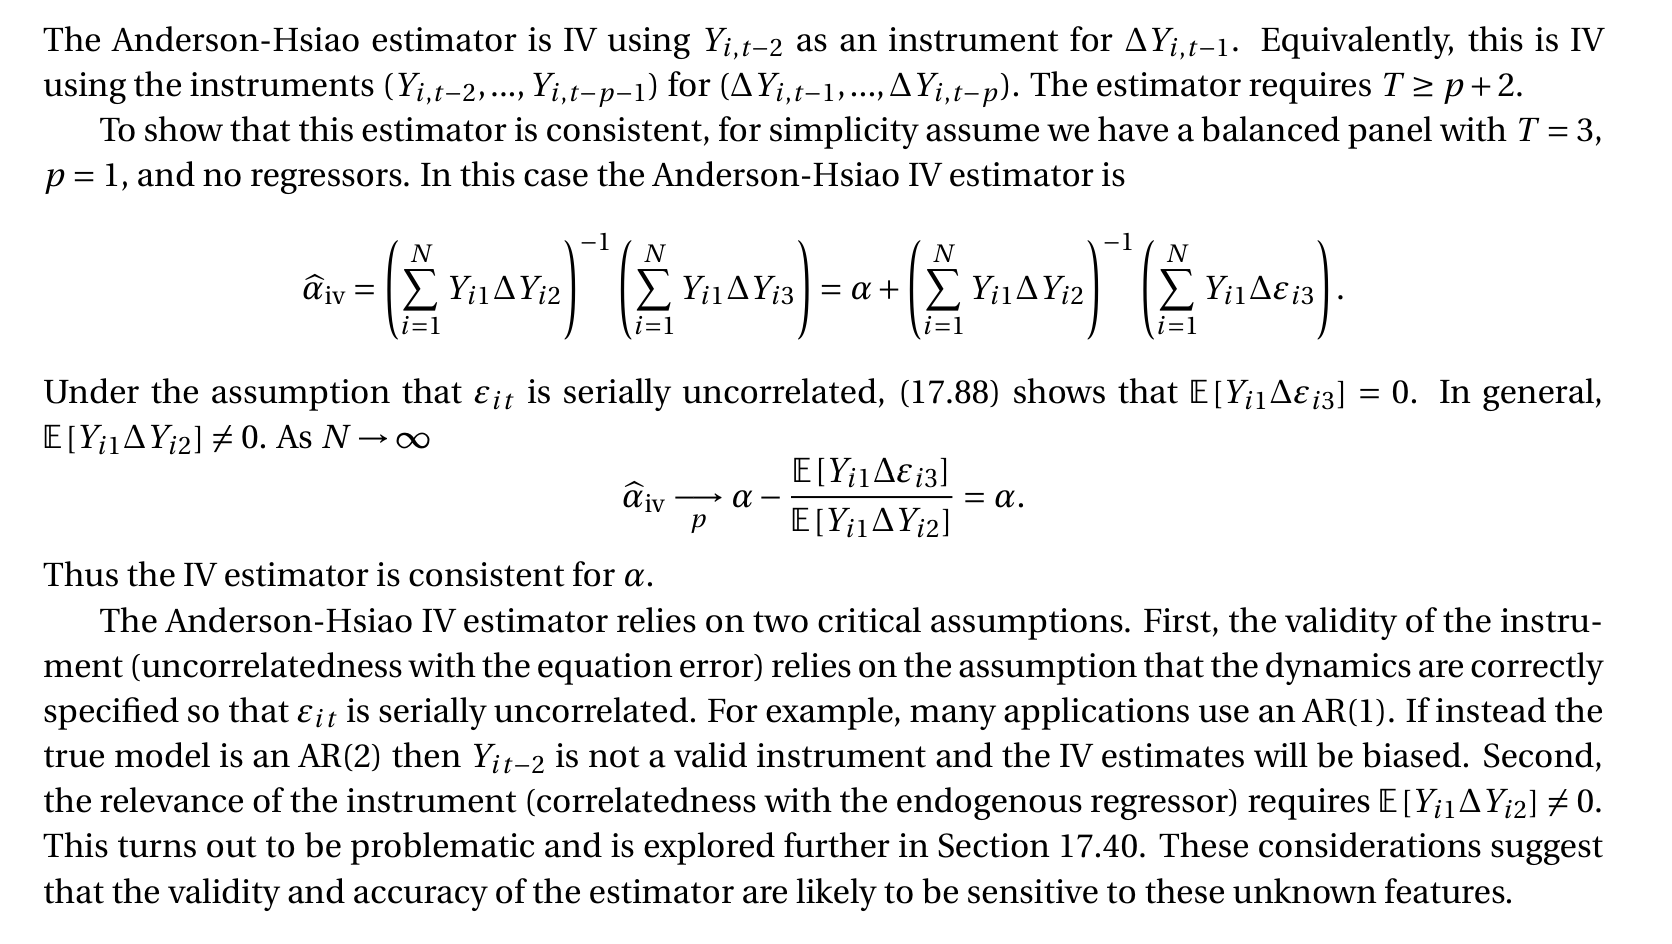
\includegraphics[width=\linewidth]{figures/Anderson-Hsiao-1981-2.png}
    \caption{Anderson and Hsiao(1981)}
\end{figure}

Using similar reasoning, other approaches use sequential exogeneity to circumvent FE meth-
ods altogether rather than to save their consistency. For example, Blundell and Bond (1998)
start from the original specification:
\[y_{it} = x_{it}^{\prime} \beta + \alpha_i + u_{it}, \]
where correlation between $\alpha_{i}$ an $x_{it}$ is suspected to be due to $y_{i,t-1}$, contained in $x_{it}.$

\begin{definition}[Blundell and Bond(1998)]
    \

    \begin{align*}
        y_{it} &= \alpha _i + \beta_1 y_{i,t-1} + u_{it} \\
        &= \beta_1 y_{i,t-1} + (u_{it} + \alpha_i) 
    \end{align*}
    Use $\Delta y_{i,t-1}$ as the IV for $y_{i,t-1}$
\end{definition}
